\documentclass[12pt]{article}
\usepackage[margin=2.5cm]{geometry}
\usepackage{enumerate}
\usepackage{amsfonts}
\usepackage{amsmath}
\usepackage{fancyhdr}
\usepackage{amsmath}
\usepackage{amssymb}
\usepackage{amsthm}
\usepackage{mdframed}
\usepackage{graphicx}
\usepackage{subcaption}
\usepackage{adjustbox}
\usepackage{listings}
\usepackage{xcolor}
\usepackage{booktabs}
\usepackage[utf]{kotex}
\usepackage{hyperref}

\definecolor{codegreen}{rgb}{0,0.6,0}
\definecolor{codegray}{rgb}{0.5,0.5,0.5}
\definecolor{codepurple}{rgb}{0.58,0,0.82}
\definecolor{backcolour}{rgb}{0.95,0.95,0.92}

\lstdefinestyle{mystyle}{
    backgroundcolor=\color{backcolour},
    commentstyle=\color{codegreen},
    keywordstyle=\color{magenta},
    numberstyle=\tiny\color{codegray},
    stringstyle=\color{codepurple},
    basicstyle=\ttfamily\footnotesize,
    breakatwhitespace=false,
    breaklines=true,
    captionpos=b,
    keepspaces=true,
    numbers=left,
    numbersep=5pt,
    showspaces=false,
    showstringspaces=false,
    showtabs=false,
    tabsize=1
}

\lstset{style=mystyle}

\pagestyle{fancy}
\renewcommand{\headrulewidth}{0.4pt}
\lhead{CSC 373}
\rhead{Worksheet 2 Solution}

\begin{document}
\title{CSC373 Worksheet 2 Solution}
\maketitle

\bigskip

\begin{enumerate}[1.]
    \item

    \begin{center}
    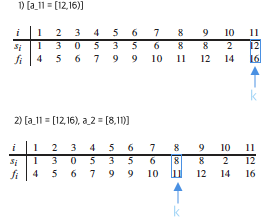
\includegraphics[width=\linewidth]{images/worksheet_2_solution_3.png}
    \end{center}

    \bigskip

    This approach is a greedy algorithm because algorithm

    \begin{enumerate}[1)]
        \item Has the greedy choice: selecting the last activity to start that is compatible
        with all previously selected activites

        \item Has the greedy choice that is always part of optimal solution:

        \bigskip

        \underline{\textbf{Claim:}}

        \bigskip

        Consider any nonempty subproblem $S_k$. Let $a_m$ be an activity in $S_k$
        with the last activity to start that is compatible with all previously selected
        activities. Then $a_m$ is included in some maximum-size subset of mutually
        compatible activities of $S_k$

        \begin{proof}
        Let $A_k$ be a maximum-size subset of mutually compatible activities in $S_k$,
        and let $a_j$ be the activity in $A_k$ with the last activity to start that is
        compatible with all previously selected activities.

        \bigskip

        If $a_j = a_m$, we are done, since we have shown that $a_m$ is the maximum-size
        subset of mutually compatible activities of $S_k$.

        \bigskip

        If $a_j \neq a_m$, let the set $A'_k = A_k = \{a_j\} \cup \{a_m\}$ be
        $A_k$ but subtituting $a_m$ for $a_j$. The activities in $A'_k$ are disjoint,
        which follow because the activities in $A_k$ are disjoint, $a_j$ is the
        first activity in $A_k$ to finish, and $s_j \leq s_m$.

        \bigskip

        Since $\lvert A'_k \rvert = \lvert A_k \rvert$, we conclude that $A'_k$
        is a maximum-size subset of mutually compatible activities of $S_k$, and it includes $a_m$.
        \end{proof}
    \end{enumerate}

    \bigskip

    \underline{\textbf{Notes:}}

    \bigskip

    \begin{itemize}
        \item Greedy Algorithm

        \begin{itemize}
            \item Always makes the choice that looks best at the moment

            \begin{itemize}
                \item Locally optimal solution leads to globally optimal solution
            \end{itemize}

        \end{itemize}

        \item Activity-selection Problem (Greedy algorithm using dynamic programming)

        \begin{itemize}
            \item Goal: Selecting maximum size set of mutually compatible activities

            \bigskip

            \underline{\textbf{Example:}}

            \bigskip

            \begin{tabular}{c|ccccccccccc}
                $i$ & 1 & 2 & 3 & 4 & 5 & 6 & 7 & 8 & 9 & 10 & 11\\
                \hline
                $s_i$ & 1 & 3 & 0 & 5 & 3 & 5 & 6 & 8 & 8 & 2 & 12\\
                $f_i$ & 4 & 5 & 6 & 7 & 9 & 9 & 10 & 11 & 12 & 14 & 16
            \end{tabular}

            \bigskip

            \item Suppose a set exists $S = \{a_1 = [s_1, f_1), a_2 = [s_2, f_2), ..., a_n = [s_n, f_n)\}$

            \begin{itemize}
                \item $a_i$ represents an $i^{th}$ activity
                \item $s_i$ represents starting time
                \item $f_i$ represents finishing time
                \item $0 \leq s_i < f_i < \infty$
                \item $a_1, ..., a_n$ sorted in monotonically increasing order of finish time

                \bigskip

                \quad i.e.

                \bigskip

                \quad $f_1 \leq f_2 \leq f_3 \leq ... \leq f_{n-1} \leq f_n$

                \bigskip

                \item $a_i$ and $a_j$ are \textbf{compatible}, if intervals $[s_i, f_i)$ and $[s_j, f_j)$
                don't overlap

                \bigskip

                \quad i.e

                \bigskip

                \quad $s_i \geq f_j$ and $s_j \geq f_i$

                \bigskip

            \end{itemize}

            \item Steps

            \begin{enumerate}[1.]
                \item Think about dynamic programming solution

                \begin{itemize}
                    \item Construct optimal solution using two subproblems

                    \begin{mdframed}

                    \textbf{$S_{ij}$:} activities that start after activity $a_i$ finishes and before
                    activity $a_j$ starts

                    \bigskip

                    i.e.

                    \bigskip

                    $S_{19} = \{a_4 = [5,7), a_6 = [5, 9), a_7 = [6, 10)\}$

                    \bigskip

                    \textbf{$A_{ij}$:} maximum set of mutually compatible activities in $S_{ij}$ (including $a_k$)

                    \begin{itemize}
                        \item $A_{ik} = A_{ij} \cap S_{ik}$
                        \item $A_{kj} = A_{ij} \cap S_{kj}$
                        \item $A_{ij} = A_{ik} \cup \{a_k\} \cup A{kj}$
                        \item So, $\lvert A_{ij} \rvert  = \lvert A_{ik} \rvert + \lvert A_{kj} \rvert + 1$
                    \end{itemize}

                    \end{mdframed}

                    \item Verify that optimal solution $A_{ij}$ must include optimal solution to the two subproblems
                    for  $S_{kj}$

                    \begin{mdframed}
                        Let $A'_{kj}$ be another mutually compatible activities in $S_{kj}$ where $\lvert A'_{kj} \rvert > \lvert A_{kj} \rvert$.

                        \bigskip

                        Then we could use $A'_{kj}$ in a solution to subproblem of $S_{ij}$

                        \bigskip

                        Then we have $\lvert A_{ik} \rvert + \lvert A'_{kj} \rvert + 1 > \lvert A_{jk} \rvert + \lvert A_{kj} \rvert + 1 = \lvert A_{ij} \rvert$ mutually compatible activites

                        \bigskip

                        This contradicts assumption that $A_{ij}$ is an optimal solution
                    \end{mdframed}

                    \item Verify that optimal solution $A_{ij}$ must include optimal solution to the two subproblems
                    for $S_{ik}$

                    \begin{mdframed}
                    The same applies for activities in $S_{ik}$
                    \end{mdframed}
                \end{itemize}

                \item Observe that only one choice - greedy choice, and that when we make the greedy choice, only one subproblem remains

                \begin{itemize}
                    \item Steps

                    \begin{enumerate}[1.]
                        \item Make a greedy choice
                        \begin{itemize}
                            \item Choose an activity that makes the most resource possible (intuition)
                            \item Choose an acitivty that finishes the earliest (intuition)
                        \end{itemize}
                        \item Solve a subproblem: Find activities that start after $a_1$ finishes
                        \item Verify that making greedy choices always arrive at optimal solution
                    \end{enumerate}
                \end{itemize}

                \bigskip

                \begin{mdframed}

                \underline{\textbf{Theorem 16.1 (Page 418):}}

                \bigskip

                Consider any non-empty subproble $S_k$, and let $a_m$ be an activity in $S_k$
                with the earliest finish time. Then $a_m$ is included in some maximum-size subset of
                mutually compatible activities of $S_k$

                \end{mdframed}
                \item Develop recursive greedy solution

                \begin{center}
                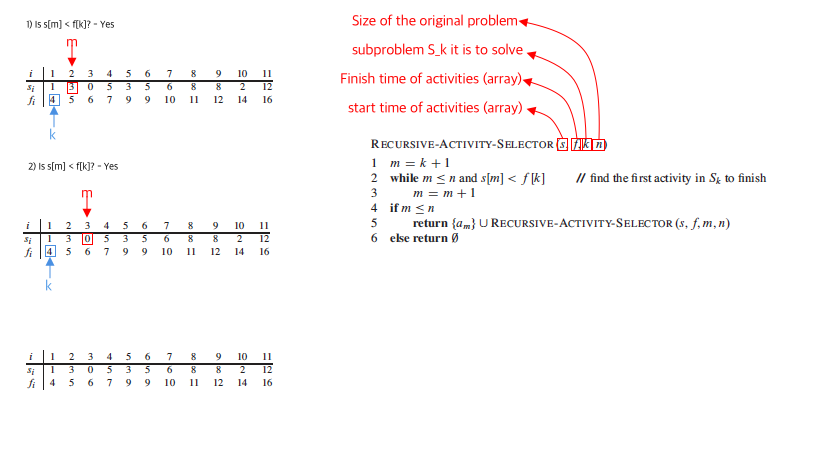
\includegraphics[width=\linewidth]{images/worksheet_2_solution_1.png}
                \end{center}


                \item Convert the recursive algorithm into iterative one

                \begin{center}
                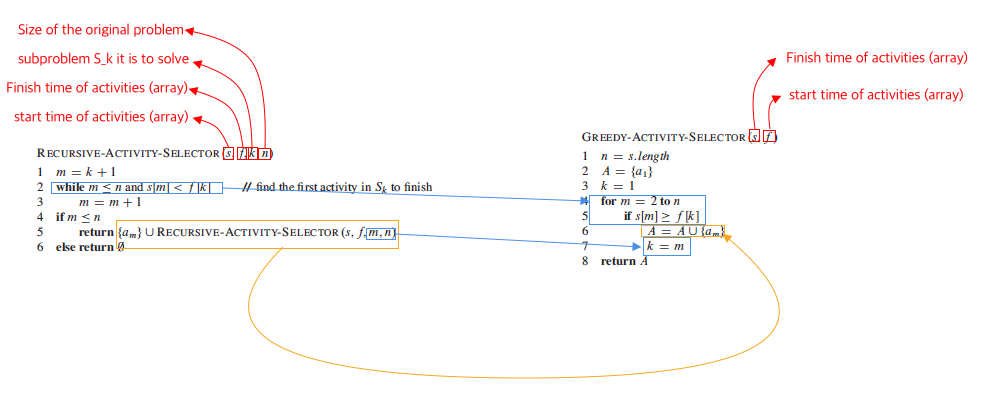
\includegraphics[width=\linewidth]{images/worksheet_2_solution_2.png}
                \end{center}
            \end{enumerate}
        \end{itemize}
    \end{itemize}

    \item

    \bigskip

    \begin{itemize}
        \item Greedy Choice

        \begin{itemize}
            \item Choose $x_i$ that is greater than the current maximum as the upper bound
            of unit length closed interval
            \item Choose $x_i$ that is smaller than the current minimum as the lower bound of unit length
            closed interval
        \end{itemize}

        \bigskip

        \underline{\textbf{Example:}}

        \bigskip

        $\{0,1,2,3,4,5\}$ $\to$ $[0,5]$

        \bigskip

        $\{0,-1,3,5,2\}$ $\to$ $[-1,5]$

        \item Optimal Substructure

        \begin{mdframed}

        \end{mdframed}

        \item Algorithm

        \begin{enumerate}[1)]
            \item Start with $[a_1, a_1]$
            \item if the size of the set is 1, then return $[a_1, a_1]$
            \item if the size of the set is greater than 2, then

            \begin{itemize}
                \item Set $i = 1$, where $i$ represents the index in the set $S$
                \item For each incrementing $i$
                \begin{itemize}
                    \item Compare $a_i$ with the value $a_{\text{currnet min}}$ in unit closed interval $[a_{\text{currnet min}},a_{\text{currnet max}}]$
                    \begin{itemize}
                        \item if $a_i < a_{\text{currnet min}}$, then replace $a_{\text{currnet min}}$ in $[a_{\text{currnet min}},a_{\text{currnet max}}]$
                        with $a_i$
                    \end{itemize}
                    \item Compare $a_i$ with the value $a_{\text{currnet max}}$ in unit closed interval $[a_{\text{currnet min}},a_{\text{currnet max}}]$

                    \begin{itemize}
                        \item if $a_i > a_{\text{currnet max}}$, then replace $a_{\text{currnet max}}$ in $[a_{\text{currnet min}},a_{\text{currnet max}}]$
                        with $a_i$
                    \end{itemize}

            \end{itemize}
            \end{itemize}
        \end{enumerate}
    \end{itemize}

    \underline{\textbf{Notes:}}

    \bigskip

    \begin{itemize}
        \item I am having difficulty providing optimal substructure to problem
        \item Unit length

        \begin{itemize}
            \item $[1,25, 2.25]$ includes all $x_i$ such that $1.25 \leq x_i \leq 2.25$.
        \end{itemize}
        \item Greedy-choice property and optimal substructure to problem are the two key ingredients
        \item Summary of Steps for Greedy Algorithm

        \begin{enumerate}[1.]
            \item Determine the optimal structure of the problem
            \item Develop a recursive solution.
            \item Show that if we make the greedy choice, then only one subproblem remains
            \item Prove that it is always safe to make the greedy choice
            \item Develop a reursive algorithm that implements the greedy strategy
            \item Convert the recursive algorithm to an iterative algorithm
        \end{enumerate}

        % \item Steps to Designing Greedy Algorithm

        % \begin{enumerate}[1.]
        %     \item Cast the optimization problem as one in which we make a choice and are left
        %     with one subproblem to solve
        %     \item Prove that there is always an optimal solution to the original problem that makes
        %     the greedy choice, so that the greedy choice is always safe
        %     \item Demonstrate optimal substructure by showing that having made the greedy
        %     choice, what remains is a subproblem with the property that if we combine an
        %     optional solution to the subproblem with the greedy choice we have made,
        %     we arrive at an optimal solution to the original problem
        % \end{enumerate}

        \item Criteria for Greedy Algorithm
        \begin{enumerate}[1.]
            \item Greedy-choice property

            \begin{itemize}
                \item Exists if we can assemble a globally optimal solution by making a
                locally optimal (greedy) choices
            \end{itemize}

            \item Optimal Substructure

            \begin{itemize}
                \item Exists if an optimal solution to the problem contains within it
                optimal solutions to subproblems.
            \end{itemize}
        \end{enumerate}

        \item Greedy vs Dynamic Programming

        \begin{itemize}
            \item 0-1 Knapsack Problem

            \begin{center}
            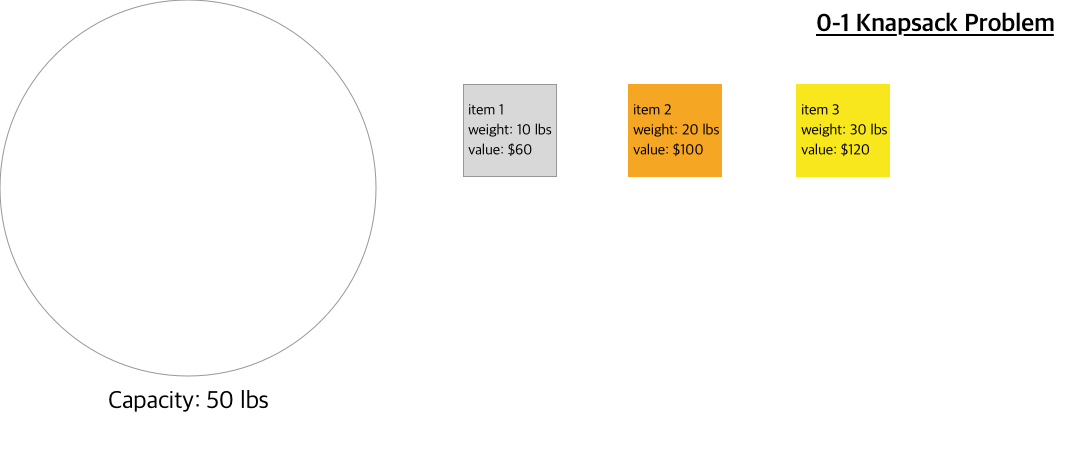
\includegraphics[width=\linewidth]{images/worksheet_2_solution_4.png}
            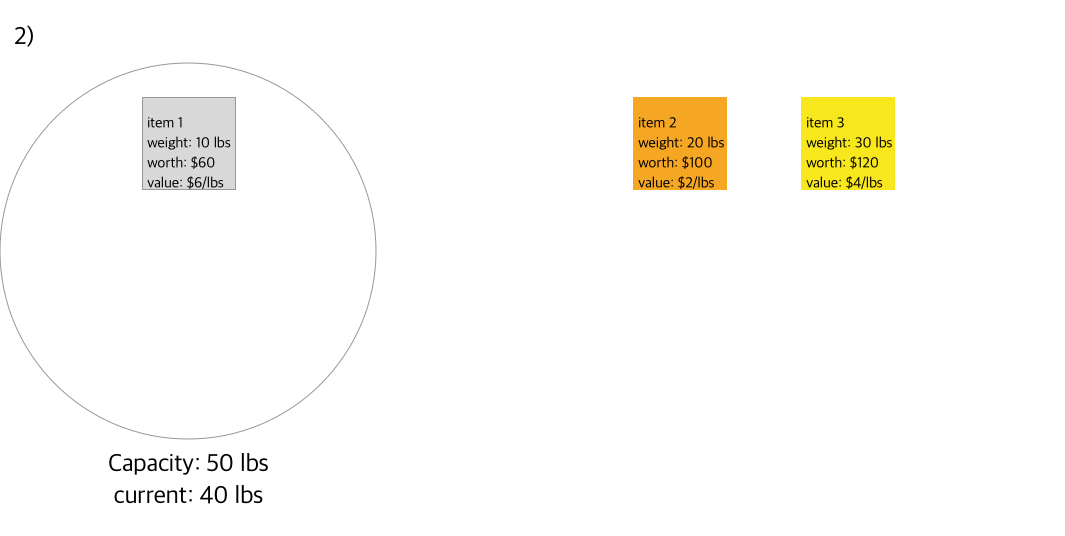
\includegraphics[width=\linewidth]{images/worksheet_2_solution_5.png}
            
\includegraphics[width=\linewidth]{images/worksheet_2_solution_6.png}
            \end{center}

            \item Fractional Knapsack Problem

            \begin{center}
            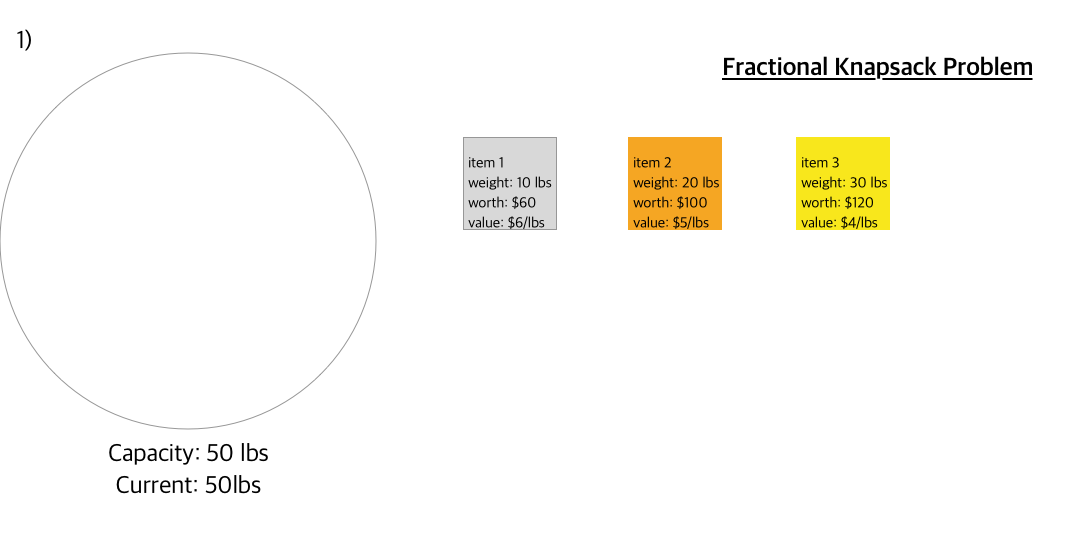
\includegraphics[width=\linewidth]{images/worksheet_2_solution_7.png}
            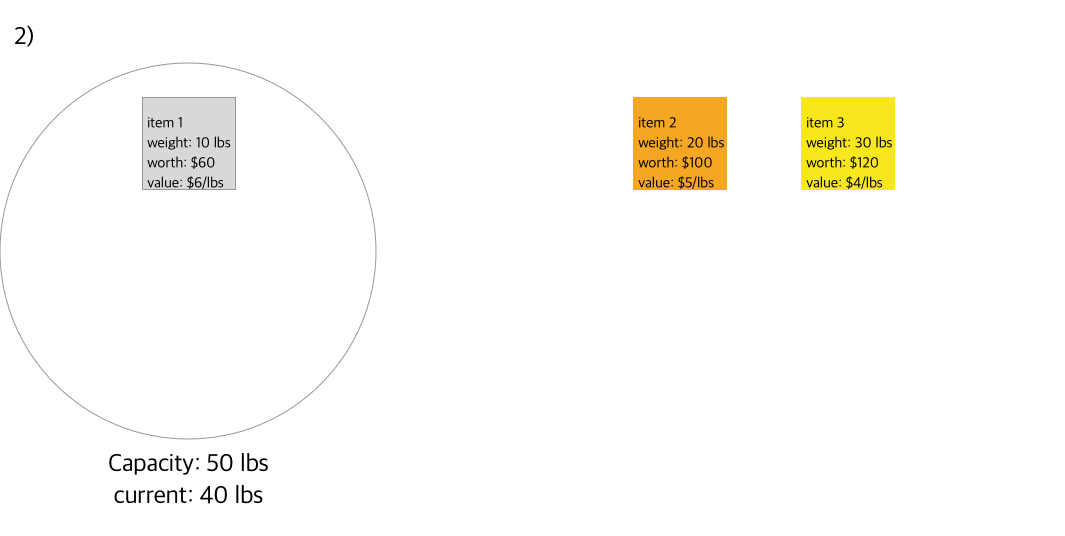
\includegraphics[width=\linewidth]{images/worksheet_2_solution_8.png}
            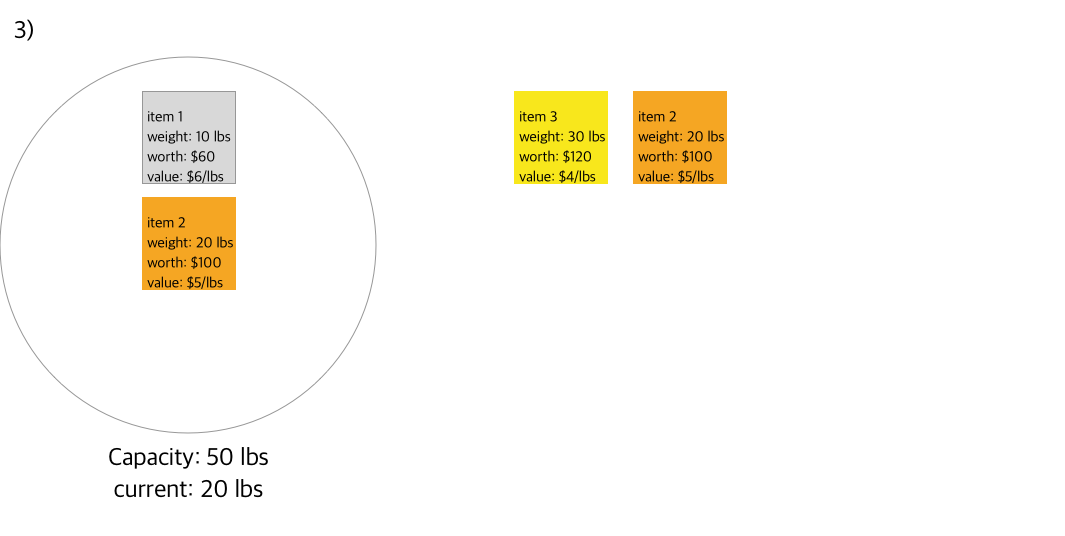
\includegraphics[width=\linewidth]{images/worksheet_2_solution_9.png}
            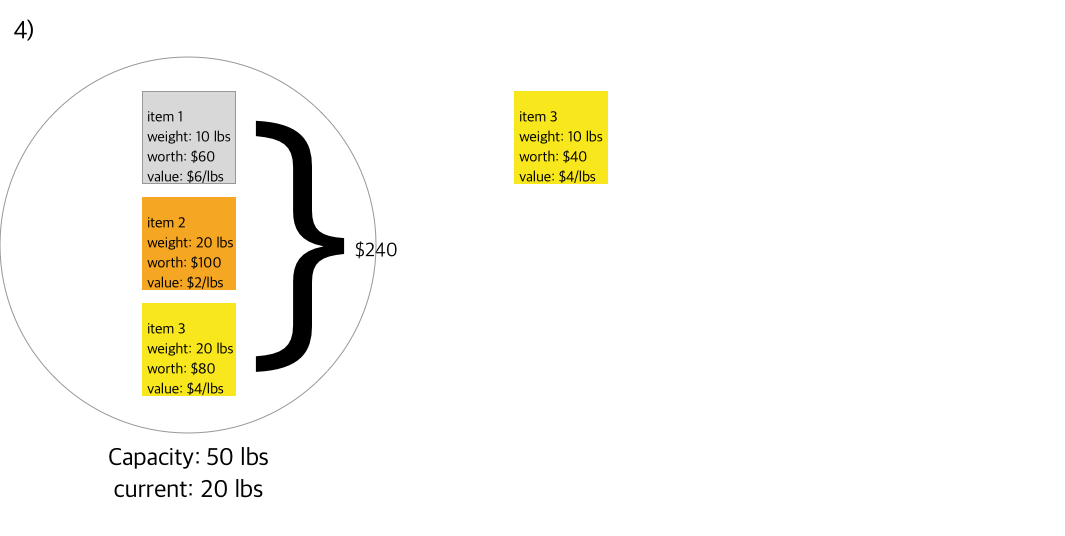
\includegraphics[width=\linewidth]{images/worksheet_2_solution_10.png}
            \end{center}
        \end{itemize}
    \end{itemize}


\end{enumerate}

\end{document}